% !TeX encoding = UTF-8
% !TeX spellcheck = es_ES
% !TeX root = ../ComponentCatalog.tex
%!TEX root=../ComponentCatalog.tex

%RJ45
\begin{table}[H]
    \centering
    \renewcommand\theadfont{\bfseries}
    \setlength{\tabcolsep}{10pt}
    \renewcommand{\arraystretch}{1.5}

    \begin{tabular}{|c|c|c|c|c|}
        \beginConnectorTable{RJ45}
        \multirow{3}{*}{\makecell{Macho}}
    
        \connectordata{
            \begin{scope}
                \clip (0,0) rectangle  +(3,1.5);
                \node[inner sep=0pt] at (1.5,0.75)
                    {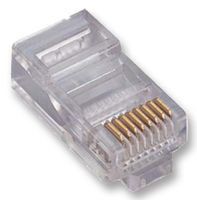
\includegraphics[scale=.1]{pictures/connectors/RJ45-nb.jpg}};
            \end{scope}
        }{
            \draw (0,0) rectangle (3,1.5) ;
        }{Amazon}{RJ45} {150V} {1.5A} 
        
        \connectorinfo{Codigo}{MTP-88-U}{
            \tabitem \textbf{Fabricante}: Multicomp
        }
        \cline{1 - 2}
        \multirow{3}{*}{\makecell{Macho}}
        \connectordata{
            \begin{scope}
                \clip (0,0) rectangle  +(3,1.5);
                \node[inner sep=0pt] at (1.5,0.75)
                    {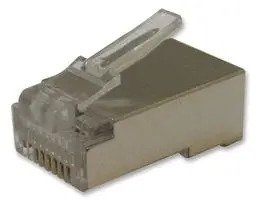
\includegraphics[scale=.1]{pictures/connectors/RJ45-b.jpg}};
            \end{scope}
        }{
            \draw (0,0) rectangle (3,1.5) ;
        }{Amazon}{RJ45} {150V} {3A}
        \connectorinfo{Codigo}{7001-8P8C-R-M}{
            \tabitem \textbf{Fabricante}: Multicomp Pro
        }
        \cline{1 - 2}
        \connectorblockinfo{Uso}{Modulos LCC OpenlCB}
        \connectorblockinfo{Ubicacion}{Terraza}
    \end{tabular}
    \caption{Conectores RJ45}
    \label{tab:RJ45}
\end{table}